\chapter{Traitement de texte 1}\label{ficheTexte1}  

\begin{itemize}
\item Logiciel\footnote{Le logiciel LibreOffice est librement téléchargeable : \url{http://www.libreoffice.org/}} : \emph{LibreOffice Writer} 
\item Prérequis : aucun
\item Matières concernées : français, anglais, sciences de la Vie et de la Terre
\item Objectifs : utiliser un traitement de texte pour mettre en forme un texte simple et l'exporter au format PDF (document rendu sur la plateforme \emph{Moodle}).
\item Compétences : 
        \begin{itemize}
        \item distinguer et mettre en forme caractères, paragraphes et pages ;
        \item insérer une image ; 
        \item exporter au format PDF.
        \end{itemize}
\item Cette fiche est à réaliser :
        \begin{itemize}
        \item avant les vacances d'octobre en français ;
        \item avant les vacances de Noël en anglais ;
        \item avant les vacances de printemps en sciences de la Vie et de la Terre. 
        \end{itemize}
\prof{\item vous devez préparer trois éléments \underline{avant} la séance : \begin{itemize}\item récupérer sur Moodle le fichier qui contient un texte simple non mis en forme sur lequel les élèves travailleront ;\item mettre à disposition des élèves sur la page Moodle de votre cours le fichier sur lequel ils travailleront ; \item créer un dossier de remise de devoir sur la page Moodle de votre classe car les élèves rendent cette activité sous la forme d'un fichier PDF déposé sur Moodle.\end{itemize} }
\end{itemize}


\section{Introduction} 

Un traitement de texte est un logiciel qui permet d'effectuer la mise en forme d'un texte : choix d'une police de caractères et de sa taille ou sa couleur, mise en forme de la page (marges) et des paragraphes, création de listes à puces et bien d'autres choses encore.

\prof{on pourra ici indiquer qu'il existe plusieurs logiciels de traitement de texte, le plus connu étant Word contenu dans le pack Office de Microsoft. Le traitement de texte utilisé ici est Writer, de la suite LibreOffice. Il présente l'avantage d'être libre et gratuit. L'utilisation de nombreuses fonctions est la même pour ces deux logiciels.}



\section{Ouvrir LibreOffice Writer}\index{Ouvrir!Writer}

Lancer le logiciel en utilisant la <<\,loupe\,>> :

\uneimageici{./images/generales/loupe}{.7\textwidth}

... puis en indiquant \emph{LibreOffice} :

\uneimageici{./images/generales/loupeRecherche}{.7\textwidth}

Choisir \emph{Document Writer} dans la liste proposée :

\uneimageici{./images/generales/fenetreOuvertureWriter}{.5\textwidth}

On arrive alors dans la fenêtre principale du traitement de texte qui contient une page blanche. Les principales icônes sont décrites ci-dessous :

\uneimageici{./images/texte/WriterPresentation}{\textwidth}

\prof{faites manipuler le logiciel aux élèves, parcourez avec eux les différentes icônes.}



%
%
%  S  É  A  N  C  E     I
%
%




\section{Séance 1 : mettre en forme un extrait de \emph{La Belle et la Bête}}\index{Writer!Mise en forme simple d'un texte}\index{Mise en forme d'un texte (Writer)}

\subsection{Ouvrir le fichier à traiter}

Sur la page \emph{Moodle} du cours, récupérer le fichier \texttt{LaBelleEtLaBete.odt}. Si nécessaire, se reporter à la fiche méthode \emph{Récupérer un document sur Moodle}, paragraphe \vref{MoodlePrendreDoc}.

Une fois le fichier enregistré sur le \emph{Bureau} de l'ordinateur, revenir dans \emph{LibreOffice Writer}, cliquer sur le menu \texttt{Fichier}, puis \texttt{Ouvrir}.

Dans les \texttt{Favoris}, choisir \texttt{Bureau}, puis cliquer sur le nom du fichier avant d'appuyer sur le bouton \texttt{Ouvrir}.      

\deuximagesPGici{./images/texte/WriterOuvrirFichier1}{\textwidth}%
                {./images/texte/WriterOuvrirFichier2}{\textwidth}





\subsection{Énoncé}

\prof{Assurez-vous que tous les élèves ont franchi les premières étapes ci-dessus. Lire ensuite l'énoncé avec les élèves et montrer le résultat attendu (affichage au TBI du résultat). À partir de ce point, les élèves travaillent chacun à leur rythme.}

\boiteEnonce{Le but de cet exercice est de mettre en forme un extrait de \emph{La Belle et la Bête}, de Jeanne-Marie Leprince de Beaumont, dont vous venez de récupérer une version <<\,brute\,>>. Le modèle à obtenir est montré ci-dessous.\newline Une fois la mise en forme terminée, vous devrez exporter votre fichier au format PDF (le fichier doit être nommé à partir de votre nom : \texttt{Nom-Prénom-date.pdf}) et le rendre sur la plateforme Moodle à l'endroit indiqué par votre enseignant.}

L'objectif est d'obtenir le résultat suivant :

\begin{center}\fbox{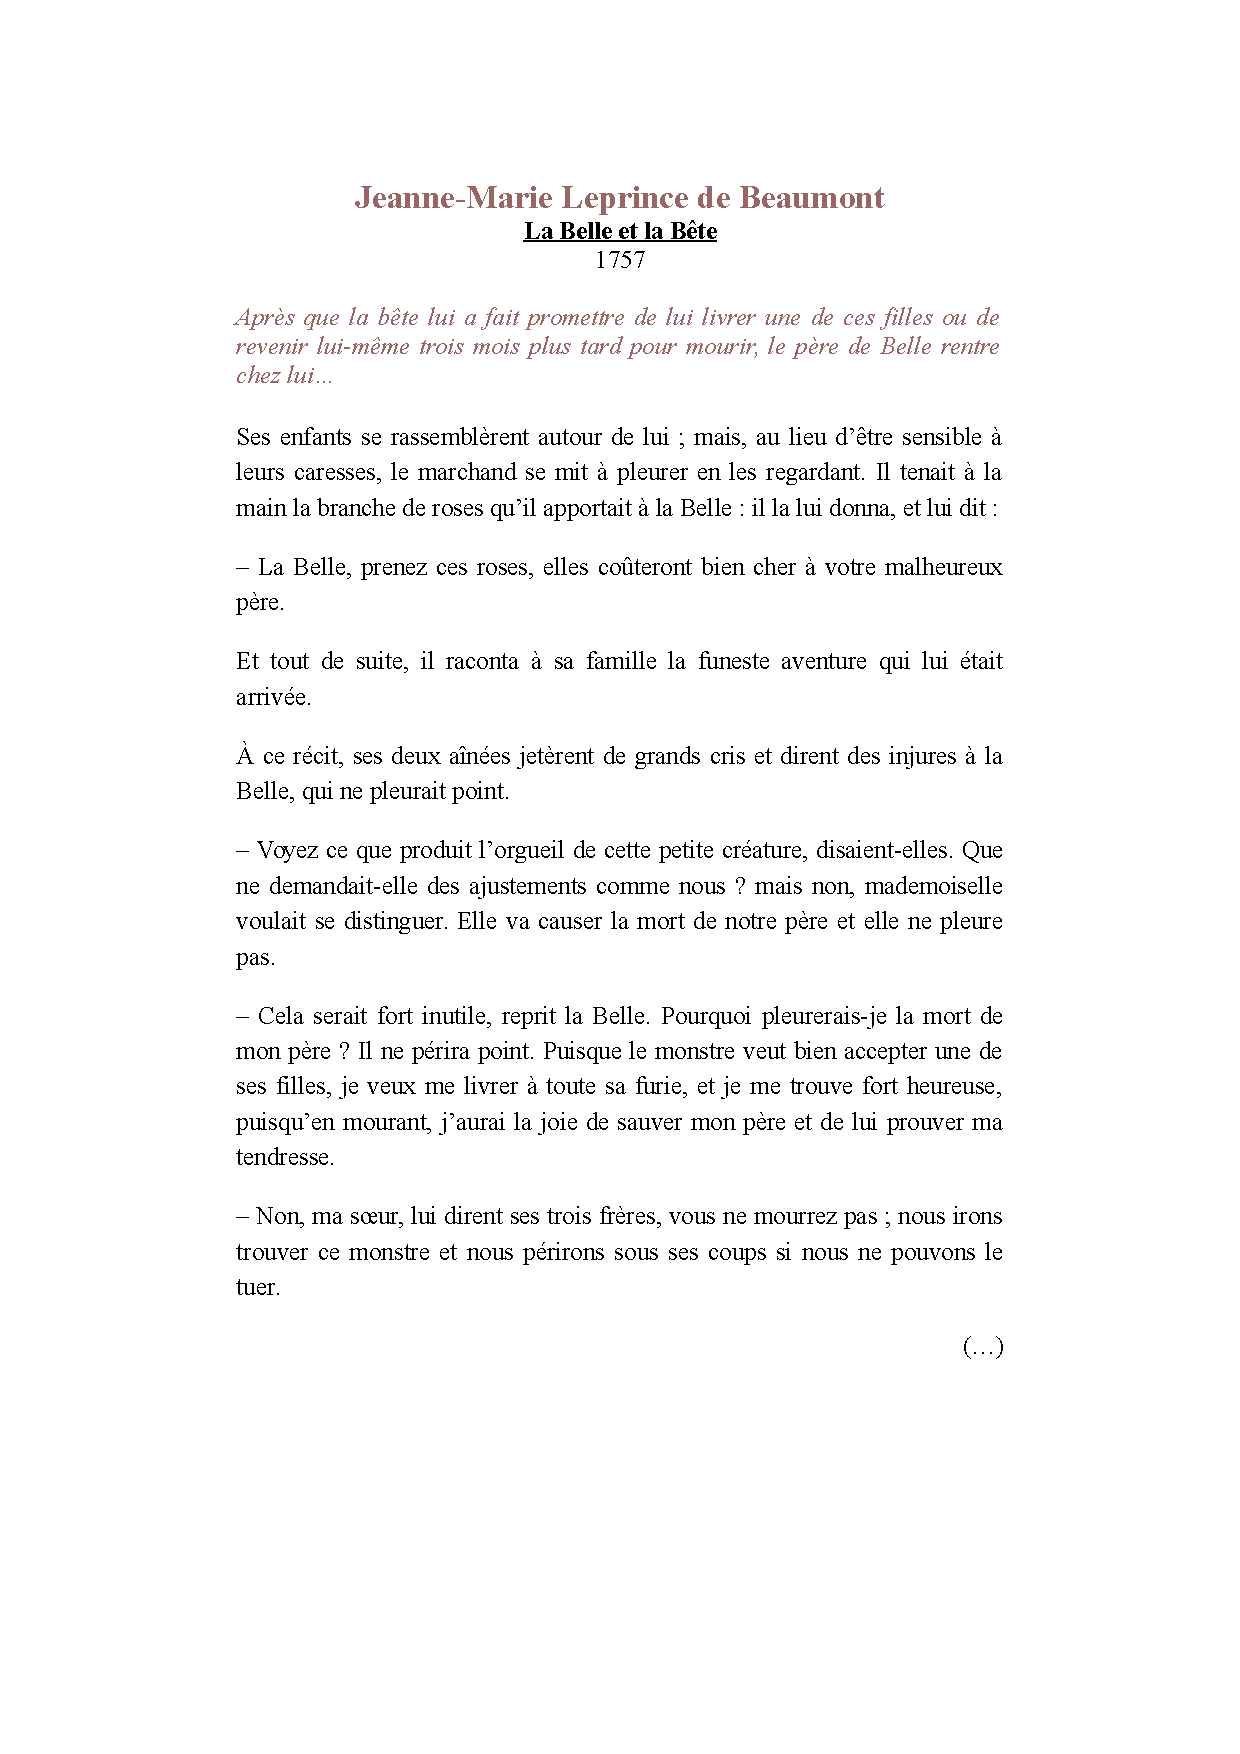
\includegraphics[width=.85\textwidth]{./sources/texte01/LaBelleEtLaBeteFormatee}}\label{modelePage}\end{center}



\subsection{Sauvegarder le fichier}\index{Writer!Enregistrer}\index{Enregistrer (Writer)}

Il est important de sauvegarder régulièrement le fichier sur lequel on travaille.

Pour enregistrer votre travail :
\begin{itemize}
\item Ouvrir le menu \texttt{Fichier}.
\item Choisir \texttt{Enregistrer sous...}
\item Choisir comme emplacement le \emph{Bureau} de l'ordinateur.
\item Entrer le nom du fichier sous la forme \texttt{Nom-Prénom-date.ods}
\end{itemize}

\uneimageici{./images/tableur/CalcEnregistrerFichier}{.8\textwidth}

Appuyer régulièrement sur la combinaison de touche \texttt{cmd} + \texttt{S} : c'est le \emph{raccourci clavier} permettant d'enregistrer votre travail.\index{Raccourci Clavier! Cmd + S, enregistrer}

\uneimageici{./images/generales/clavierCmdS}{.5\textwidth}








\subsection{Mettre en forme la page}\index{Writer!Marges}\index{Marges (Writer)}

Pour commencer on définit la taille des quatre marges du document (gauche, droite, haut et bas). On choisit ici 4\,cm à gauche et à droite, et 3\,cm en haut et en bas.

Dans le menu \texttt{Format}, choisir \texttt{Page...} :    

\uneimageici{./images/texte/WriterFormatMenu}{.3\textwidth}

Dans la boîte de dialogue qui s'ouvre, se rendre dans l'onglet \texttt{Page} puis régler les marges :  

\uneimageici{./images/texte/WriterBoiteMarge}{.7\textwidth}











\subsection{Choisir une police de caractères}\index{Writer!Changer la police de caractères}\index{Police de caractère (Writer)}

Par défaut, la police de caractères du document est \texttt{Liberation Serif}. On souhaite passer à \texttt{Times New Roman}. La première étape est de sélectionner tout le texte. Pour cela :

\begin{itemize}
\item soit, on passe par le menu \texttt{Édition} et on choisit \texttt{Tout sélectionner} ;
\item soit, on utilise le raccourci clavier \texttt{cmd + A}.\index{Raccourci Clavier! Cmd + A, sélectionner tout (Writer)}    
\end{itemize}

\deuximagesici{./images/texte/WriterEditionMenuSelectAll}{.7\textwidth}
              {./images/generales/clavierCmdA}{.7\textwidth}

Dans la liste déroulante des polices de caractères (1 dans l'image ci-dessous), choisir la police \texttt{Times New Roman} : le texte sélectionné change alors de police de caractères.  


\uneimageici{./images/texte/WriterChangePolice}{.7\textwidth}


\subsection{Modifier la taille des caractères}\index{Writer!Taille des caractères}\index{Tailles des caractères (Writer)} 

Avant de modifier la taille des caractères, il faut sélectionner les parties du texte à modifier. On choisit une taille de 12 points pour le texte (on peut utiliser \texttt{cmd + A} pour tout sélectionner ou passer par le menu \texttt{Édition}) et 16 pour le titre (à sélectionner à la souris avant le changement de taille).

\deuximagesici{./images/texte/WriterChangeTailleCaractere1}{\textwidth}%
              {./images/texte/WriterChangeTailleCaractere2}{\textwidth}







\subsection{Centrer du texte}\index{Writer!Centrer le texte}\index{Centrer le texte (Writer)}

Pour centrer les trois premières lignes, il faut tout d'abord les sélectionner à l'aide de la souris. Cliquer ensuite sur le bouton \emph{Centrer horizontalement} : 

\uneimageici{./images/texte/WriterCentrerTitre}{.7\textwidth}

%%%%%%%%%%%%%%%%%%%%%%%%%%%%%%%%%%%%%%%%%%%%%%%%%%%%%%%%%%
%\subsection{Créer une liste à puces}\index{Writer!Liste à puces}\index{Liste à puces (Writer)}   
%
%Les différents personnages de l'acte 1 scène 1 sont présentés sous la forme d'une liste où chaque ligne démarre par un $\bullet$ qui s'appelle une \emph{puce}. L'ensemble est nommé \emph{liste à puces}.   
%
%Pour créer une liste à puce, sélectionner les lignes concernées puis cliquer sur le bouton \emph{Activer les puces}.
%
%\uneimageici{./images/texte/WriterListePuce}{.7\textwidth}
%%%%%%%%%%%%%%%%%%%%%%%%%%%%%%%%%%%%%%%%%%%%%%%%%%%%%%%%%%%




\subsection{Souligner du texte}

On souligne le titre.\index{Writer!Souligner}\index{Souligner (Writer)} Pour cela, on le sélectionne, puis on applique une des deux méthodes suivantes :

\begin{itemize}
\item utilisation du bouton \emph{souligner} :  
\uneimageici{./images/texte/WriterSouligne}{.7\textwidth}
\item utilisation du raccourci clavier \texttt{cmd + U} :\index{Raccourci Clavier! Cmd + U, souligner (Writer)} 
\uneimageici{./images/generales/clavierCmdU}{.3\textwidth}
\end{itemize}




\subsection{Mettre un texte en gras ou en italique}

Pour mettre du texte en gras ou en italique\index{Writer!Gras}\index{Gras (Writer)}\index{Writer!Italique}\index{Italique (Writer)}, il faut tout d'abord le sélectionner, puis appliquer une des deux méthodes suivantes :

% attention, ci-dessous j'ai fait deux listes à puces différentes pour pouvoir conserver 
% une pleine largeur pour les images...
\begin{itemize}
\item utilisation du bouton \emph{gras} ou \emph{italique} :
\end{itemize}
\deuximagesici{./images/texte/WriterFonteGrasse}{\textwidth}%
              {./images/texte/WriterTexteItalique}{.9\textwidth}
\begin{itemize}
\item utilisation du raccourci clavier \texttt{cmd + B} (gras) ou \texttt{cmd + I} (italique)\index{Raccourci Clavier! Cmd + I, italique (Writer)}\index{Raccourci Clavier! Cmd + B, gras (Writer)} :
\end{itemize}
\deuximagesici{./images/generales/clavierCmdB}{.7\textwidth}%
              {./images/generales/clavierCmdI}{.7\textwidth}


    









\subsection{Modifier la couleur des caractères} 


On change la couleur du titre\index{Writer!Changer la couleur des caractères}\index{Couleur des caractères (Writer)}. Pour cela, on le sélectionne, puis on choisit la couleur désirée (par exemple \emph{Rouge 8}) :

\uneimageici{./images/texte/WriterCouleurPolice}{.5\textwidth}










\subsection{Mettre en forme des paragraphes}\index{Writer!Interligne}\index{Writer!Espacement entre paragraphes}\index{Interligne (Writer)}\index{Espacement entre paragraphes (Writer)} 



Il faut tout d'abord sélectionner tous les paragraphes sur lesquels on veut appliquer un changement.

Comme l'espace entre les lignes est une propriété du paragraphe, on peut le modifier en passant par le menu \texttt{Format} puis \texttt{Paragraphe...}

On va modifier deux propriétés : 
\begin{itemize}
\item l'espace entre deux lignes au sein d'un même paragraphe (\emph{interligne}) ;
\item l'espace entre deux paragraphes (\emph{espacement sous le paragraphe}).
\end{itemize}


\uneimageici{./images/texte/WriterMiseEnFormeParagraphe1}{.8\textwidth}

Dans la boîte de dialogue qui s'ouvre, se rendre dans l'onglet \texttt{Retraits et espacement}, puis régler l'interligne et l'espacement sous le paragraphe :  

\uneimageici{./images/texte/WriterMiseEnFormeParagraphe2}{.8\textwidth}







\subsection{Justifier un paragraphe}\index{Writer!Justifier}\index{Justifier (Writer)}\index{Aligner le texte à droite et à gauche (justifier) (Writer)}

Lorsque le texte est aligné à la fois du côté gauche et du côté droit, on dit qu'il est \emph{justifié}. Pour justifier les parties du texte qui doivent l'être:

\begin{itemize}
\item sélectionner les paragraphes à justifier à l'aide de la souris
\item cliquer sur le bouton \emph{justifié} ou utiliser le raccourci clavier \texttt{cmd + J}. 
\end{itemize}

\uneimageici{./images/texte/WriterParagrapheJustifie}{.8\textwidth}





\subsection{Aligner à droite}  

Pour terminer, on aligne à droite les points de suspension finaux. Pour cela, il faut les sélectionner à l'aide de la souris puis cliquer sur le bouton \texttt{Aligner à droite} :  

\uneimageici{./images/texte/WriterAlignerADroite}{\textwidth}



\subsection{Exporter au format PDF}\index{Writer!Exporter au format PDF}\index{PDF (exporter au format) (Writer)}

Une fois le travail achevé et sauvegardé, il faut exporter le fichier au format PDF. Pour cela, deux solutions :
\begin{itemize}\item passer par le menu \texttt{Fichier} et choisir \texttt{Exporter au format PDF...} Les réglages proposés par défaut dans la boîte de dialogue conviennent. Appuyer sur \texttt{Exporter}, puis terminer en cliquant sur \texttt{Enregister}.\end{itemize} 

\deuximagesPGici{./images/texte/WriterMenuFichier}{.7\textwidth}%
                {./images/texte/WriterBoiteExportPDF}{\textwidth}

\begin{itemize}\item utiliser le bouton \texttt{Export direct au format PDF} :\end{itemize} 
\uneimageici{./images/texte/WriterIconePDF}{.3\textwidth}

Dans les deux cas, le fichier PDF est enregistré au même endroit que le fichier sur lequel on travaille.


\cadre{Le \textbf{format PDF} est un format parfaitement adapté aux échanges de documents : il est non modifiable et lisible sur tous les périphériques (ordinateurs, tablettes, smartphones). Il peut contenir du texte, des images, des liens vers l'internet et même des vidéos ou du son. \newline À chaque fois qu'il faut rendre ou envoyer un document qui n'est pas destiné à être modifié, il faut privilégier le format de fichier PDF.}  








\subsection{Remettre le travail achevé sur Moodle}

Une fois votre travail terminé et exporté au format PDF, il faut le remettre au professeur. Pour cela, se connecter à la page \emph{Moodle} du cours. Chercher le dossier de remise de devoir (icône 
\includegraphics[width=.04\textwidth]{./images/methode/MoodleDevoirIcone1}), puis remettre le devoir. Si nécessaire, se reporter à la fiche méthode \emph{Remettre un devoir sur Moodle}, paragraphe \vref{MoodleRendreDevoir}.  





\subsection{Pour aller plus loin...}  

Quand les textes deviennent très longs, il est difficile d'y retrouver un mot en particulier. Les traitements de texte disposent donc d'un outil permettant de rechercher un mot.\index{Writer!Rechercher}\index{Rechercher (Writer)} 

Lorsqu'on souhaite retrouver un mot dans une page de texte, on peut utiliser le raccourci clavier \texttt{cmd + F} :\index{Raccourci Clavier! Cmd + F, rechercher (Writer)}   

\uneimageici{./images/generales/clavierCmdF}{.35\textwidth}

Une barre de recherche s'ouvre alors en bas de la fenêtre :

\uneimageici{./images/texte/WriterBarreRecherche}{.9\textwidth}

Essayer de rechercher le mot \emph{Belle} : il suffit d'entrer le mot dans la zone de saisie (2 sur l'image ci-dessus) puis d'appuyer sur la touche \texttt{Entrée}. Les flèches (3 sur l'image ci-dessus) permettent de passer d'un mot trouvé à l'autre. Pour fermer la barre de recherche, cliquer sur la croix (1 sur l'image ci-dessus).   


%%%%%%%%%%%%%%%%%%%%%%%%%%%%%%%%%%%%%%%%%
%\subsubsection{Remplacer les : par des .}\index{Writer!Rechercher et remplacer}\index{Rechercher et remplacer (Writer)}
%
%\uneimageici{./images/texte/WriterEditionMenu}{.35\textwidth}
%
%\uneimageici{./images/texte/WriterBoiteRechercherRemplacer}{.5\textwidth}
%%%%%%%%%%%%%%%%%%%%%%%%%%%%%%%%%%%%%%%%%



%
%
%  S  É  A  N  C  E     II
%
%


\section{Séance 2 : mettre en forme un texte de J. Swift}\label{ficheTexte2}

\prof{l'anglais est enseigné en groupes de niveau et il était difficile de trouver un texte qui soit valable pour tous les groupes. N'hésitez pas à vous approprier cette séance en proposant votre propre texte à votre groupe. Si vous souhaitez faire cette activité avec un texte différent, il suffit de fournir aux élèves (i) le texte brut non mis en forme, (ii) le modèle à atteindre. Ainsi vous pourrez mieux intégrer cette séance à votre progression.}  



\boiteEnonce{Le but de cet exercice est de mettre en forme un extrait d'une œuvre de Jonathan Swift, \emph{Gulliver's travels}, dont une version <<\,brute\,>> est disponible sur la page Moodle de votre cours. Le modèle à obtenir est montré ci-dessous. Pour parvenir à ce résultat, vous devrez utiliser deux nouvelles fonctionnalités du traitement de texte : passer le texte en majuscule et encadrer un paragraphe. \\ Une fois la mise en forme terminée, vous devrez exporter votre fichier au format PDF (le fichier doit être nommé à partir de votre nom : \texttt{Nom-Prénom-date.pdf}) et le rendre sur la plateforme Moodle à l'endroit indiqué par votre enseignant.}

L'objectif est d'obtenir le résultat suivant :

\begin{center}\fbox{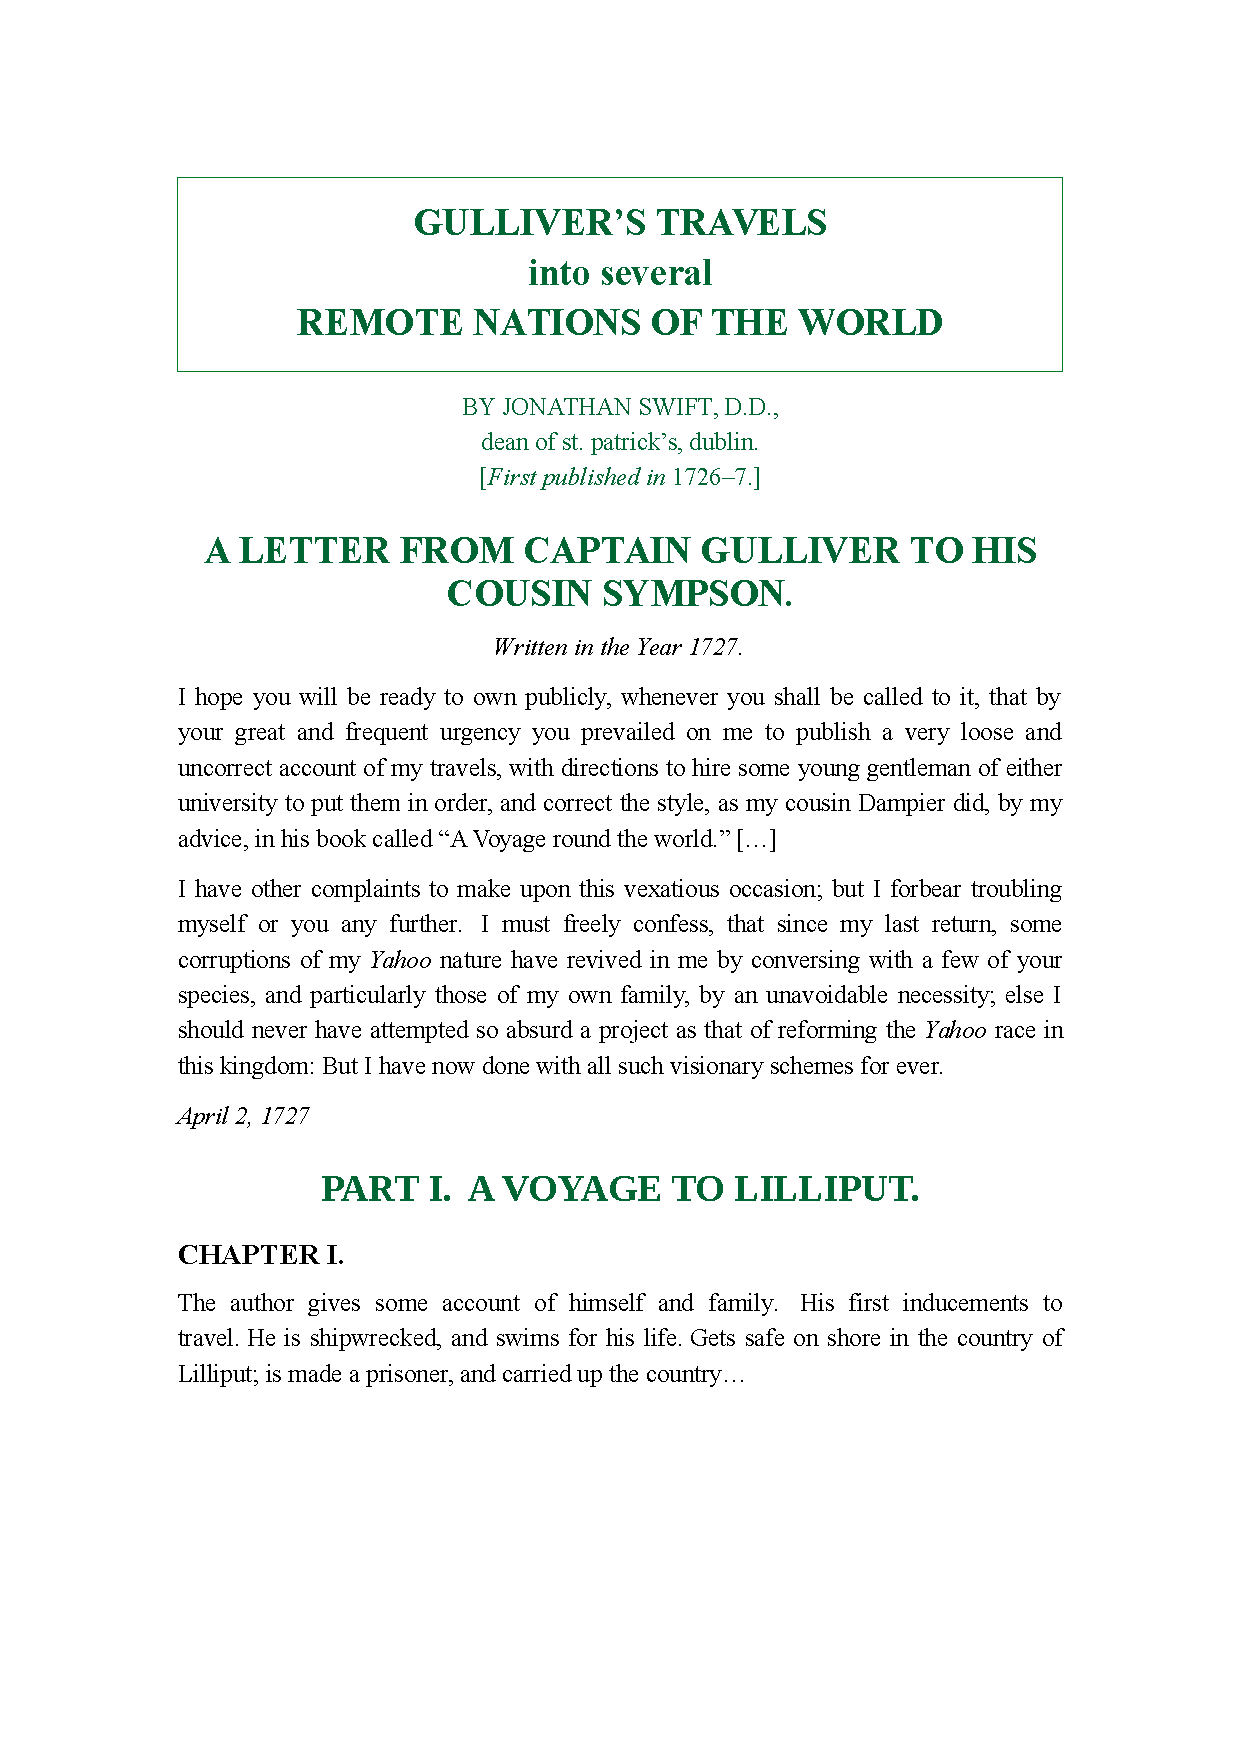
\includegraphics[width=.75\textwidth]{./sources/texte01/ExtraitGulliver6eFormate}}\label{modelePage}\end{center}


Les opérations à effectuer pour y parvenir sont les suivantes :

\begin{itemize}
\item marges de 3\,cm à gauche, à droite, en haut et en bas ;
\item police de caractères \emph{Times New Roman} ;  
\item titres en caractères de taille 16 points et de couleur \emph{Turquoise} ;
\item texte en caractères de taille 12 points avec un interligne fixe de 0,6\,cm et un espace sous les paragraphes de 0,25\,cm ;
\item quelques parties du texte en italique ; 
\item le texte justifié et les titres centrés.
\end{itemize}


\subsection{Passer le texte en majuscule}\index{Writer!Majuscule}\index{Majuscule (Writer)}

Certaines parties du texte doivent être écrites en majuscules. Pour cela, sélectionner-les\footnote{On peut sélectionner différents endroits du texte en même temps en maintenant la touche \texttt{Cmd} enfoncée pendant qu'on sélectionne les zones à la souris.} puis ouvrir le menu \texttt{Format} et choisir \texttt{Caractère...} Une boîte de dialogue s'ouvre : dans l'onglet \texttt{Effet de caractère}, il faut choisir \texttt{Majuscules}, puis cliquer sur \texttt{OK}.  

\uneimageici{./images/texte/WriterTexteMajuscule}{.9\textwidth}









\subsection{Encadrer un paragraphe}\index{Writer!Encadrer}\index{Encadrer (Writer)} 

Pour encadrer le titre de l'ouvrage et ajouter un espacement entre le texte et la bordure qui l'entoure, on utilise l'outil \emph{bordures de paragraphe}. Pour cela, sélectionner le titre, puis ouvrir le menu \texttt{Format} et choisir \texttt{Paragraphe...} Une boîte de dialogue s'ouvre : dans l'onglet \texttt{Bordures}, modifier les propriétés des bordures comme indiqué ci-dessous, puis cliquer sur \texttt{OK}.

\uneimageici{./images/texte/WriterParagrapheEncadre}{.9\textwidth}



\subsection{Pour aller plus loin...}

Une fois votre document rendu au format PDF sur la page \emph{Moodle} de votre cours, amusez-vous à découvrir toutes les propriétés des paragraphes. Vous pouvez par exemple ajouter :
\begin{itemize}
\item un retrait pour le premier mot du paragraphe ;
\item un retrait pour le paragraphe en entier ; 
\item un arrière plan (une couleur de fond) ;
\item une ombre derrière le paragraphe ; 
\item divers types de bordures. 
\end{itemize}


%
%
%  S  É  A  N  C  E     III
%
%


\section{Séance 3 : mettre en forme un compte rendu d'expérience}\label{ficheTexte3}

\prof{cette séance doit être faite sur deux périodes si les élèves préparent eux-mêmes leur compte rendu d'expérience (une période pour la rédaction du compte rendu, et une pour la mise en forme). Il est également possible (comme pour les séances 1 et 2 ci-dessus) de leur donner le compte rendu de la dernière expérience faite, mais non mis en forme, ainsi qu'un modèle de ce qui est attendu. Il faut prévoir une image à insérer dans le compte rendu (format JPG ou PNG), et la mettre à disposition des élèves sur la page \emph{Moodle} de votre cours. Précisez aux élèves vos attentes : mise en page, alignements, espacements, taille des caractères, etc.}  

\boiteEnonce{Le but de cet exercice est de mettre en forme un compte rendu d'expérience et d'y insérer une image fournie par votre professeur. Vous devez utiliser les techniques apprises dans cette fiche sur le traitement de texte pour préparer votre document.\newline Une fois la mise en forme terminée, vous devrez exporter votre fichier au format PDF (le fichier doit être nommé à partir de votre nom : \texttt{Nom-Prénom-date.pdf}) et le rendre sur la plateforme Moodle à l'endroit indiqué par votre enseignant.}


\subsection{Insérer une image}\index{Writer!Insérer une image}\index{Insérer une image (Writer)}

La première étape est de récupérer sur la page \emph{Moodle} du cours l'image à insérer dans le compte rendu. Si nécessaire, se reporter à la fiche méthode \emph{Récupérer un document sur Moodle}, paragraphe \vref{MoodlePrendreDoc}.

\vspace{12pt}

Pour insérer une image dans un document texte :

\begin{enumerate}
\item Cliquer sur la souris pour positionner le curseur à l'endroit où l'image doit être insérée et sauter quelques lignes pour laisser de la place à l'image :

\uneimageici{./images/texte/WriterInsertionImage2}{.6\textwidth}

\item Se rendre dans le menu \texttt{Insertion} et choisir \texttt{Image...}

\uneimageici{./images/texte/WriterInsertionImage1}{.6\textwidth}

\item Dans la boîte de dialogue qui s'ouvre, rechercher le fichier qui contient l'image et terminer l'insertion en cliquant sur \texttt{Ouvrir}.

\item L'image peut alors être redimensionnée :
        \begin{itemize}
        \item soit, en utilisant les poignées qui apparaissent lorsqu'on clique sur l'image ;
        \uneimageici{./images/texte/WriterInsertionImage3}{.5\textwidth}
        \item soit, en double-cliquant sur l'image pour faire apparaître la boîte de dialogue suivante. Il faut dans un premier temps cocher la case \texttt{Conserver le ratio}, puis on peut régler les dimensions souhaitées pour l'image.
        \uneimageici{./images/texte/WriterInsertionImage4}{.7\textwidth}
        \end{itemize}
\end{enumerate}


